\chapter{JetBrains MPS}
\label{chap:jetbrains_mps}

Before we can dive into the problem itself, we need to give readers a good understanding of how the target environment works.
We will walk through some basic features of the JetBrains MPS~\cite{MPS} so that we know what the goal of this thesis is.
\\

JetBrains is a company with a long history of IDE (Integrated Development Environment) development.
Some of their tools, such as IntelliJ IDEA\footnote{https://www.jetbrains.com/idea/} or Resharper\footnote{https://www.jetbrains.com/resharper/}, are widely used by professionals around the world and are considered to be top quality products.
Their project called MPS (Meta Programming System) is a development environment, that allows building custom domain specific languages or extending existing ones.
Developers can use these newly created languages inside MPS and, out of their programs, they can generate actual code in a given target language such as Java.
The project itself started in 2003 as a research project, but JetBrains have been using it in the development of their own products since 2006.
It is being developed as an open-source product under the Apache 2.0 license.
\\

In this chapter, we will explain fundamental basics of MPS as it is crucial in the understanding of what we are trying to achieve in this thesis.

\section{Abstract syntax tree}
At the first sight, MPS might look like a typical IDE, but it differs from the rest in one important aspect.
MPS does not work with the textual representation of the code as usual, but rather with its AST (abstract syntax tree), that is the model of the code.
The code itself, which is later compiled and run, is built out of this tree.
So when users are creating programs using MPS, they are basically assembling the tree out of defined building blocks of the language.
The definition of the language used dictates, which statements or elements can be nested inside each other and what structure the AST can have.
\\

Keeping the model of the code in the AST form has several advantages.
One of them is, that  MPS then only allows composing the program strictly following the syntax of the language, which results in an inability to actually write syntactically invalid code.
It is generated out of the always-valid AST beyond user's reach.
This is extremely handy when used, for example, for educational purposes, as you can guide students through code creation easily using auto-completion or other tools available.
It also means that MPS understands the code much better and is able to perform some interesting actions or refactoring.
\\

After the program's tree is assembled like this, there can be rules defined on how to generate code out of that tree.
These defined generators can target any language and, possibly, we can transform this model into more different languages' models if such generators exist.
This generated code can then be for example platform dependent, but the model itself is not tied to any specific platform or environment.
This mechanism gives us, for instance, the possibility to extend existing languages easily and to create various syntactic sugar, targeting the same language again, but hiding complicated mechanisms from the user.

\section{Projectional editor}
As stated before, MPS is not an ordinary tool, but its most distinctive feature might be the projectional editor.
The projectional editor is the place where “interaction” between the code and the programmer takes place.
The idea behind projectional editing is following.
When the user is not working with the text source code directly, as usual, every node of the AST can be represented in any form and take any shape.
It is just up to the designer of the language what shape will each node take inside the projectional editor.
For a better understanding, we will give a small example.
\\

Let's assume we have a language with typical if/else structure similar to the one in Java:

\begin{center}
	\begin{minipage}{.38\textwidth}
		\begin{alltt}
			if (\textit{condition})
			    \textit{then statement block}
			else
			    \textit{else statement block}
		\end{alltt}
	\end{minipage}
\end{center}

\vspace{3mm}

Its abstract syntax tree representation then might look something like shown on Figure \ref{fig:if_ast}.
\\

\begin{figure}[h]
	\centering
	\includegraphics[scale=0.75]{./img/if_statement_ast.png}
	\caption{"If statement" abstract syntax tree}
	\label{fig:if_ast}
\end{figure}

The underlying child nodes have their own children and so on.
Their type is narrowed down by the language structure definition (meaning that we restrict the condition to be an expression, statement block to be a list of statements, etc.).
\\

Now, the representation of code inside the projectional editor can have any visual form and is not bound to the textual representation at all.
It can be a text-like representation similar to what we are used to or for example blocks of both branches can be aligned next to each other like shown in Figure \ref{fig:if_editor}.
\\

\begin{figure}[h]
	\centering
	\hspace{-4mm}
	\includegraphics[scale=0.75]{./img/if_statement_editor.png}
	\caption{"If statement" projectional editor example}
	\label{fig:if_editor}
\end{figure}

We have an absolute free will in how do we design each node of the AST.
We can style the node graphically and define its layout in any way.
This, of course, comes with some drawbacks such as designing a representation like this is quite complicated, even for a human.
\\

For a definition of concept's appearance, JetBrains have developed a cellular system that allows placing concept's properties and children into different cells.
These cells then can be styled to user's liking.
There are many different types of cells, each behaving a little bit different towards its contents.
We are talking about various horizontal or vertical lists etc.
More extra cells can be added on top of that holding no content but specifying additional layout adjustments such as indentation.
Each cell can have special context menus bound to it, its formatting can be customized and so on.
In Figure {\ref{fig:if_editor_definition})}, you can see what a real editor definition might look like for the if statement of the BaseLanguage language.

\section{Languages and solutions}

The editor itself breaks up into two main parts --- language and solution editors.
The former is used for language definition, where we model languages' structure.
The latter one then imports these MPS languages and enables the user to write code using them.
Multiple languages can be used together inside one solution, effectively combining their features into one project.

\subsection{Plugin solutions}

Users can also create a "plugin solution" which is a special kind of solution, that can also import languages, but more importantly can tamper with the MPS editor itself.
It is able to introduce elements inside the MPS such as menu items, window panels and more.
The big advantage of MPS is that everything is happening live and just by mere regeneration (rebuilding) of a plugin solution, changes are immediately incorporated without the need of restarting the IDE.
Plugin solutions are important in this thesis and were used to accomplish an important part of the work as later described.

\section{Creating a language in MPS}

This section will illustrate how a language is created inside MPS, what elements make it up and what needs to be done in order to make the language usable.
\\

Main building blocks of any MPS language are concepts.
You can imagine they are the nodes of the AST and we build the code out of them.
Every concept can have a definition of one or more different editor aspects.
Every aspect defines the concept from a different point of view.
One aspect might say where the concept in AST can be included, another one what code is generated out of it and so on.
Concepts took over some design patterns known from object oriented programming.
The concept can be inherited from a parent (abstract) concept and it can implement a special interface concept.
Most importantly, concepts have child concepts and that is how the AST itself is created.
\\

We will describe some of these aspects more closely, as it will give the reader better understanding of the problem, that is being solved.
Some are less important for our cause, some are vital.

\subsection{Structure aspect}

The structure aspect is the most important aspect, as all concepts must be first defined here.
This aspect treats the concept somewhat like a Java class.
User can define the name, inheritance, interfaces and concept fields:

\begin{itemize}
	\item \textbf{Children} -- a list of child concepts and their cardinality

	\item \textbf{References} -- a list of references to already existing nodes (e.g. think reference to a node of a method in a method call statement)

	\item \textbf{Properties} -- arbitrary fields of any type that can hold value, just like class fields in Java
\end{itemize}

The concept can be further marked as a \textit{rootable} one, which means it can be a top level element for some code in a given language.
In Figure \ref{fig:if_statement_structure}, you can see the structure aspect definition for the if statement.

\begin{figure}[h]
	\centering
	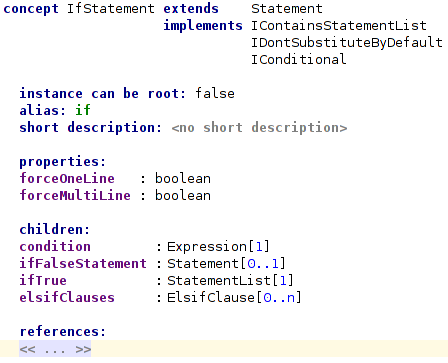
\includegraphics[scale=0.75]{./img/if_statement_structure.png}
	\caption{"If statement" structure aspect definition}
	\label{fig:if_statement_structure}
\end{figure}

\subsection{Editor aspect}
\label{chap:about_editor_aspect}

Editor aspect is where the user defines what the projectional editor representation of a code fragment (an AST node) looks like.
The user usually incorporates all children, references, and properties inside the representation so that future user of the language can insert their value into these placeholders.
Any other static components can be included too.
All elements can be styled using a language similar to CSS.
If editor concept is not defined, MPS will provide a default one that stylizes the concept into a JSON-like form, displaying all its fields nested in a JSON-like object.
This provides basic ability to use the concept when coding but it is not very user-friendly.

\begin{figure}[h]
	\centering
	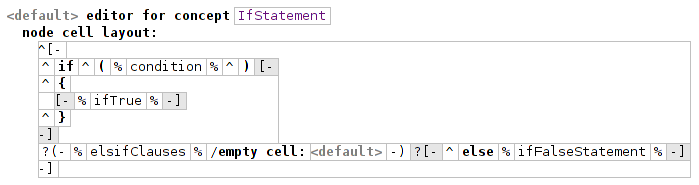
\includegraphics[width=\textwidth]{./img/if_statement_editor_definition.png}
	\caption{"If statement" editor aspect definition}
	\label{fig:if_editor_definition}
\end{figure}

\subsection{TextGen aspect}
The TextGen aspect is a one we also care about.
It defines how a certain node will be translated into a text source code.
This will allow us to generate source code in text form out of an AST model and ultimately to generate a text program out of the code user writes in the imported language.
\\

The TextGen aspect is basically just one method definition for each concept of the language.
This method has several parameters such as the currently processed node and some contextual information.
It is, however, not returning a string as perhaps expected, but rather manipulates an output buffer/stream using some built-in functions.
MPS then calls this method for the root concept of the program and it is up to this concept's TextGen method to append its children into the stream by calling their TextGen methods.
Again, we included an example of the if statement (Figure \ref{fig:if_statement_textgen}).

\begin{figure}[h]
	\centering
	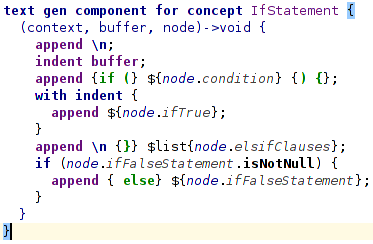
\includegraphics[scale=0.70]{./img/if_statement_textgen.png}
	\caption{"If statement" TextGen aspect definition}
	\label{fig:if_statement_textgen}
\end{figure}

\subsection{Other aspects}
Other aspects, that can be found inside MPS, are not interesting for us from this thesis' point of view.
They are mostly high level and very complicated aspects such as type checking or data-flow analysis (unreachable code detection etc.).
Creating these automatically and programmatically wouldn't be possible without human intervention as the information needed just isn't contained inside the grammar file.
These aspects will be used for adjusting the imported language and improving the usability of the language.